\documentclass[12pt,a4paper]{article}
\usepackage[top=1in,bottom=1in,left=1.5in,right=1in]{geometry}
\usepackage{mathptmx} % Times New Roman
\usepackage{setspace}
\usepackage{titlesec}
\usepackage{amsmath,amssymb}
\usepackage{cite}
\usepackage{hyperref}
\usepackage{booktabs}
\usepackage{tabularx}
\usepackage{array}
\usepackage{tikz}
\usetikzlibrary{shapes.geometric,arrows.meta,positioning,calc,decorations.pathreplacing}

\setstretch{1.5} % 1.5 line spacing per AKGEC departmental guidelines
\pagestyle{plain} % Page numbering at bottom

% Heading formatting per college guidelines: Main heading 14pt Bold, Sub-heading 12pt Bold
\titleformat{\section}{\fontsize{14pt}{17pt}\bfseries}{\thesection}{1em}{}
\titleformat{\subsection}{\fontsize{12pt}{15pt}\bfseries}{\thesubsection}{1em}{}
\titleformat{\subsubsection}{\fontsize{12pt}{15pt}\bfseries}{\thesubsubsection}{1em}{}

\setlength{\parindent}{0pt}
\setlength{\parskip}{6pt}

\begin{document}

\section*{7. System Architecture and Workflow}

\subsection*{7.1 Architectural Overview and Multi-Tier Decomposition}
The IntelliTwin framework is structured around a decoupled, multi-tier cyber-physical research architecture designed to resolve the pervasive gap between data-driven Remaining Useful Life (RUL) estimation, finite-sample distribution-free uncertainty calibration, and sequential operational maintenance decision-making [1]--[3]. In industrial rotating machinery, such as commercial turbofan aircraft engines, standard point predictions optimize symmetric statistical metrics that fail to reflect asymmetric downtime losses ($C_{\text{FAIL}} \gg C_{\text{PM}}$) [1], [5]. Concurrently, digital twin implementations in manufacturing literature frequently prioritize high-fidelity 3D geometric visualizations or centralized SCADA dashboards without mathematically formalizing how predictive uncertainty should govern discrete intervention decisions [2], [13], [14].

To bridge these disjoint paradigms, IntelliTwin decomposes asset monitoring, prognostic estimation, uncertainty calibration, and maintenance simulation into five modular, decoupled architectural tiers:
\begin{enumerate}
    \item \textbf{Tier 1: Data Ingestion and Anti-Leakage Preprocessing Tier}: Ingests multi-sensor run-to-failure streams from the NASA C-MAPSS corpus, enforces immutable engine-level disjoint split isolation, performs invariant sensor pruning, fits training-only normalization parameters, clusters operational settings, and constructs causal sliding lookback windows [1].
    \item \textbf{Tier 2: Prognostic Base Inference Tier}: Houses complementary shallow gradient-boosted decision trees (\texttt{HistGradientBoostingRegressor}) and deep recurrent neural networks (PyTorch \texttt{LSTM}), generating continuous point predictions of Remaining Useful Life [3], [4].
    \item \textbf{Tier 3: Hierarchical Conformal Calibration Tier}: Computes asymmetric nonconformity scores, evaluates exact engine-weighted quantiles under cluster exchangeability, stratifies calibration bounds across operational flight regimes, and inverts scores into finite-sample prediction intervals $[L_i(t), U_i(t)]$ targeting 90\% nominal coverage [7], [9].
    \item \textbf{Tier 4: Sequential Decision and Maintenance Simulation Tier}: Evaluates dynamic cycle-by-cycle stopping rules $\tau_i = \inf \{ t \ge W : L_i(t) \le \theta \}$ against conservative lower conformal bounds, tracks economic lifecycle expenditures in Standardized Cost Units (SCU), executes matched-conservatism attribution controls, and conducts 10,000 cluster bootstrap hypothesis tests [5], [8], [12].
    \item \textbf{Tier 5: Digital Twin Synchronization and Presentation Tier}: Formulates a real-time trace-driven state replication engine (\texttt{TwinReplayEngine}) adhering to ISO 23247 principles [14], guarantees strict numerical verification parity ($\text{atol} \le 10^{-4}$) against offline batch execution, and exposes streaming REST endpoints via FastAPI to an interactive HTML5/JavaScript operator dashboard [2], [13].
\end{enumerate}

\subsubsection*{Physical Integration and Research Demarcation}
In alignment with rigorous academic reporting standards, the physical integration boundary of the IntelliTwin system is explicitly demarcated:
\begin{itemize}
    \item \textbf{Offline Trace-Driven Simulation}: The architecture operates on historical run-to-failure telemetry from the NASA C-MAPSS simulator [1]. No live turbofan engine is physically connected to the host system, and no hardware IoT sensor bus (e.g., MQTT, OPC UA) is claimed.
    \item \textbf{Advisory Decision Support}: Maintenance orders dispatched by the simulation tier represent advisory recommendations for maintenance engineers; closed-loop physical actuation (e.g., automatic engine shutdown or thrust throttling) is strictly out of scope.
    \item \textbf{Strict Anti-Leakage Boundary}: Held-out test trajectories are isolated from model training, hyperparameter grid search, and conformal score calibration. True failure times and oracle RUL values are revealed exclusively to offline evaluation routines for post-hoc scoring.
\end{itemize}

\subsection*{7.2 Data Ingestion, Normalization, and Causal Windowing Pipeline}
The data pipeline ingests raw continuous multi-sensor records and transforms them into standardized tensor and vector representations while strictly eliminating temporal and inter-engine data leakage.

\subsubsection*{C-MAPSS Data Schema and Invariant Channel Pruning}
The raw C-MAPSS dataset provides 26 columns per cycle: engine unit identifier, cycle index, 3 operational flight condition settings, and 21 thermo-mechanical degradation sensors [1]. Across multi-regime datasets (FD002, FD004), a systematic variance audit identified six invariant or uninformative channels exhibiting zero variance or uninformative responses across all regimes:
\begin{equation}
\mathcal{S}_{\text{dropped}} = \{ s_1 \text{ (T2)}, s_5 \text{ (P2)}, s_6 \text{ (P15)}, s_{10} \text{ (epr)}, s_{16} \text{ (farB)}, s_{19} \text{ (Nf\_dmd)} \}
\end{equation}
Excluding these uninformative channels eliminates matrix rank deficiency and numerical instability. The retained schema comprises $d = 17$ informative channels: 3 operating settings ($z_1, z_2, z_3$) and 14 dynamic thermo-mechanical sensors (temperatures, pressures, core/fan speeds, fuel ratios, and coolant bleeds).

\subsubsection*{Strict Engine-Level Split Partitioning}
To prevent inter-engine correlation leakage, partitioning is strictly enforced at the engine unit level. For each benchmark dataset, entire run-to-failure engine trajectories belong exclusively to one split:
\begin{itemize}
    \item \textbf{FD001 (Single-Regime Control)}: 100 total engines split into 50 Training, 20 Calibration, 10 Validation, and 20 Test engines.
    \item \textbf{FD002 (Multi-Regime Primary)}: 260 total engines split into 130 Training, 52 Calibration, 26 Validation, and 52 Test engines.
    \item \textbf{FD004 (Multi-Regime / Multi-Fault Robustness)}: 249 total engines split into 124 Training, 50 Calibration, 25 Validation, and 50 Test engines.
\end{itemize}

\subsubsection*{Training-Only Normalization and Regime Clustering}
Standardization parameters (mean $\boldsymbol{\mu}_{\text{train}}$ and population standard deviation $\boldsymbol{\sigma}_{\text{train}}$, computed with `ddof=0`) are derived solely from the designated Training engines:
\begin{equation}
\tilde{\mathbf{x}}_i(t) = \frac{\mathbf{x}_i(t) - \boldsymbol{\mu}_{\text{train}}}{\boldsymbol{\sigma}_{\text{train}} + \epsilon}
\end{equation}
where $\epsilon = 10^{-8}$ prevents division by zero. For multi-regime sub-corpora (FD002, FD004), operating settings $(z_1, z_2, z_3)$ are standardized and clustered into $K = 6$ operational regimes ($C_1$ to $C_6$) via K-means clustering ($K = 6, \text{random\_state} = 2026, \text{n\_init} = 10$) fitted exclusively on training data, preserving deterministic centroid ordering.

\subsubsection*{Causal Sliding-Window Formulation}
To preserve temporal causality, feature representations are constructed using a fixed sliding lookback window of length $W = 30$ cycles with stride 1:
\begin{equation}
\mathbf{X}_i(t) = \begin{bmatrix}
\tilde{\mathbf{x}}_i(t - W + 1) \\
\tilde{\mathbf{x}}_i(t - W + 2) \\
\vdots \\
\tilde{\mathbf{x}}_i(t)
\end{bmatrix} \in \mathbb{R}^{W \times d} = \mathbb{R}^{30 \times 17}
\end{equation}
For early operational cycles ($1 \le t < W = 30$), the causal buffer is filling; zero padding is strictly forbidden, and prognostic inference is deferred until cycle $t = 30$. Dual feature representations are constructed from this window:
\begin{itemize}
    \item \textbf{Sequential Tensor}: A 2D matrix $\mathbf{X}_i(t) \in \mathbb{R}^{30 \times 17}$ preserving temporal ordering for the recurrent LSTM network.
    \item \textbf{Flattened Vector}: A 1D vector $\mathbf{v}_i(t) = \text{vec}(\mathbf{X}_i(t)) \in \mathbb{R}^{510}$ flattened in C-order (row-major) for gradient-boosted decision trees.
\end{itemize}

\subsection*{7.3 Prognostic Base Inference Tier}
The prognostic inference tier transforms causal window representations into continuous point estimates of Remaining Useful Life $\hat{y}_i(t)$.

\subsubsection*{Dual Target Conventions}
During base model training, Remaining Useful Life targets are clamped at an upper threshold $R_{\text{max}} = 125$ cycles:
\begin{equation}
y_{\text{train}, i}(t) = \min(R_{\text{max}}, T_i - t)
\end{equation}
reflecting the empirical physical reality that initial operational wear does not exhibit measurable degradation signatures during early component life [1]. In contrast, during held-out test evaluation, the true uncapped linear degradation target $y_{\text{eval}, i}(t) = T_i - t$ is preserved to assess genuine lifetime prognostic accuracy.

\subsubsection*{Model Architecture Workflows}
Two diverse, complementary model families are trained and frozen under Architecture Decision Record ADR-018:
\begin{itemize}
    \item \textbf{HistGradientBoostingRegressor (GBR)}: Ingests flattened 510-dimensional vectors $\mathbf{v}_i(t)$. Optimizes the asymmetric pinball loss function $\mathcal{L}_{\rho}(y, \hat{y}) = \max(\rho(y - \hat{y}), (1 - \rho)(\hat{y} - y))$ across quantiles $\rho \in \{0.05, 0.50, 0.95\}$ with histogram-binned split finding (max bins $= 255$, learning rate $= 0.05$, max leaf nodes $= 31$, L2 reg $= 1.0$).
    \item \textbf{PyTorch Deep Bidirectional LSTM}: Ingests sequential tensors $\mathbf{X}_i(t) \in \mathbb{R}^{30 \times 17}$. Features two stacked bidirectional LSTM recurrent layers ($h = 64$ hidden units per direction, 128 concatenated), variational recurrent dropout ($p = 0.20$), and a LeakyReLU projection head. Optimized using AdamW ($\eta = 10^{-3}$, weight decay $= 10^{-4}$) under Mean Squared Error loss with cosine annealing scheduling.
\end{itemize}
Point predictions are non-negatively clipped: $\hat{p}_i(t) = \max(0, \hat{y}_i(t))$. A total of 30 model checkpoints (3 datasets $\times$ 2 architectures $\times$ 5 seeds `[2026..2030]`) are registered and frozen.

\subsection*{7.4 Hierarchical Conformal Calibration and Interval Inversion Workflow}
The conformal calibration tier converts raw point predictions into statistically guaranteed, finite-sample prediction intervals $\mathcal{C}_{1-\alpha}(\mathbf{X}_i(t)) = [L_i(t), U_i(t)]$ targeting nominal 90\% coverage ($1 - \alpha = 0.90$) [4], [7], [9].

\subsubsection*{Asymmetric Decision-Aware Nonconformity Scoring}
To penalize hazardous overestimation ($\hat{y} > y$, risking in-service failure) more heavily than premature underestimation ($\hat{y} < y$, resulting in early inspection), nonconformity scores incorporate state-dependent dynamic scaling [7]:
\begin{equation}
\sigma(\hat{p}) = \left(1 + \frac{\hat{p}}{125}\right)^\gamma, \quad z(\hat{p}) = \exp\left(-\frac{\hat{p}}{20}\right)
\end{equation}
\begin{equation}
a(\hat{p}) = \sigma(\hat{p}) \cdot \exp(\beta \cdot z(\hat{p})), \quad b(\hat{p}) = \sigma(\hat{p}) \cdot \exp(-\beta \cdot z(\hat{p}))
\end{equation}
\begin{equation}
s_i(t) = \max\left( \frac{\hat{p}_i(t) - y_i(t)}{a(\hat{p}_i(t))}, \frac{y_i(t) - \hat{p}_i(t)}{b(\hat{p}_i(t))}, 0 \right)
\end{equation}
with candidate parameters $\gamma = 2$ and $\beta = -\ln 2 \approx -0.693147$, optimized via grid search on the Validation split.

\subsubsection*{Exact Engine-Weighted Quantile Solver}
To resolve the clustered temporal autocorrelation of repeated observations within engines, each observation $(i, t)$ from calibration engine $i \in \{1, \dots, m\}$ is assigned weight $w_{i,t} = \frac{1}{(m+1) \cdot n_i}$. Total finite probability mass equals $\frac{m}{m+1}$, with the remaining $\frac{1}{m+1}$ assigned to $+\infty$ [9]:
\begin{equation}
F_{\text{dev}}(q) = \frac{1}{m+1} \sum_{i=1}^m \left[ \frac{1}{n_i} \sum_{t=1}^{n_i} \mathbb{I}(s_{i,t} \le q) \right]
\end{equation}
The conformal quantile $\hat{q}_{1-\alpha}$ is the smallest observed calibration score satisfying $F_{\text{dev}}(\hat{q}_{1-\alpha}) \ge 1 - \alpha$. When calibrating within specific operational flight regimes $k \in \{1, \dots, K\}$, condition-adaptive thresholds $\hat{q}_{1-\alpha}^{(k)}$ are computed; if a regime cluster contains fewer than $m_g \ge 10$ calibration engines, fallback routing to the global threshold $\hat{q}_{1-\alpha}^{(\text{global})}$ is automatically triggered.

\subsubsection*{Closed-Form Prediction Interval Inversion}
Given the calibrated threshold $\hat{q}_{1-\alpha}$, the finite-sample prediction interval is evaluated via closed-form inversion:
\begin{equation}
L_i(t) = \max(0, \hat{p}_i(t) - \hat{q}_{1-\alpha} \cdot a(\hat{p}_i(t))), \quad U_i(t) = \hat{p}_i(t) + \hat{q}_{1-\alpha} \cdot b(\hat{p}_i(t))
\end{equation}
where $L_i(t)$ represents the conservative lower bound on Remaining Useful Life that directly drives downstream maintenance policies.

\subsection*{7.5 Discrete-Event Sequential Maintenance Utility Simulation Workflow}
The simulation tier models asset lifecycle progression cycle-by-cycle using a discrete-event simulator (\texttt{src/intellitwin/simulator/engine.py}) [5], [8].

\subsubsection*{Sequential Stopping Policy}
At each operational cycle $t \ge 30$, the simulator evaluates the lower conformal bound $L_i(t)$. When the lower bound breaches an operational threshold $\theta$ (with default $\theta = 1.0$ cycle), a preventive maintenance order is dispatched immediately:
\begin{equation}
\tau_i = \inf \{ t \ge W : L_i(t) \le 1.0 \}
\end{equation}
If $\tau_i < T_i$, planned maintenance is successfully executed at cycle $\tau_i$, terminating the trajectory without in-service incident. If the engine reaches its terminal cycle before maintenance is triggered ($\tau_i \ge T_i$), an unscheduled catastrophic failure occurs at cycle $T_i$.

\subsubsection*{Standardized Cost Units (SCU) Evaluation}
Total simulated lifecycle cost for engine $i$ is calculated under the primary reference scenario:
\begin{equation}
\text{Cost}_i(\tau_i) = \begin{cases}
C_{\text{PM}} + C_{\text{WASTE}} \cdot (T_i - \tau_i), & \text{if } \tau_i < T_i \text{ (Planned Maintenance)} \\
C_{\text{FAIL}}, & \text{if } \tau_i \ge T_i \text{ (Unscheduled In-Service Failure)}
\end{cases}
\end{equation}
with economic parameters: planned overhaul $C_{\text{PM}} = 1.0$ SCU, in-service failure penalty $C_{\text{FAIL}} = 5.0$ SCU, and wasted component life penalty $C_{\text{WASTE}} = 0.20$ SCU per cycle.

\subsubsection*{Controlled Attribution Protocol}
To verify that cost reductions stem from genuine uncertainty calibration rather than heuristic over-conservatism, outcomes are evaluated against three pre-registered matched-conservatism control families:
\begin{enumerate}
    \item \textbf{Uniformly Widened Intervals ($\delta$-Widened)}: $\hat{q}' = \hat{q} + \delta$.
    \item \textbf{Point Safety Margins ($\Delta$-Margin)}: $\hat{p}'(t) = \hat{p}(t) - \Delta$.
    \item \textbf{Earlier Scheduled Intervention ($\theta$-Offset)}: $\theta' = \theta + \tau_{\text{advance}}$.
\end{enumerate}
Statistical significance is established via 10,000 engine-level cluster bootstrap draws under Bonferroni family-wise error rate control ($\alpha = 0.0125$) and Two One-Sided Tests (TOST) non-harm equivalence bounds [12].

\subsection*{7.6 Digital Twin State Synchronization and Replay Engine}
To translate scientific models into an interactive operational prototype, IntelliTwin implements a real-time trace-driven Digital Twin synchronization engine (\texttt{TwinReplayEngine}) in \texttt{src/intellitwin/twin/replay.py} [2], [13], [14].

\subsubsection*{Thread-Safe Replay State Machine}
The replay engine manages asset state transitions through an explicit lifecycle state machine protected by mutual exclusion locks:
\begin{itemize}
    \item \textbf{WARMING\_UP (Cycles $1 \dots 29$)}: Sensor frames are buffered into the causal history. Inference is deferred; no prediction bounds or maintenance actions are emitted.
    \item \textbf{ACTIVE (Cycles $30 \dots \min(\tau_i, T_i - 1)$)}: The engine maintains the active $30 \times 17$ sliding window, applies training Z-scores, computes dual GBR/LSTM forecasts, derives conformal bounds $[L_i(t), U_i(t)]$, calculates dynamic Health Index $\text{HI}_i(t) = \min(1.0, \frac{\hat{p}_i(t)}{125})$, and evaluates maintenance policy rules.
    \item \textbf{MAINTAINED (Cycle $\tau_i$)}: Triggered when $L_i(t) \le 1.0$. The session locks, records a planned overhaul event, and halts further telemetry advancement.
    \item \textbf{FAILED (Cycle $T_i$)}: Reached if cycle $t$ attains total failure cycle $T_i$ without intervention. Records catastrophic failure and terminates the session.
\end{itemize}

\subsubsection*{Numerical Parity Verification}
To guarantee that real-time replay does not introduce numerical artifacts or windowing drift, the replay engine is audited against offline batch execution:
\begin{equation}
\max_{t} | \hat{p}_{\text{stream}}(t) - \hat{p}_{\text{batch}}(t) | \le 10^{-4}, \quad \max_{t} | L_{\text{stream}}(t) - L_{\text{batch}}(t) | \le 10^{-4}
\end{equation}
Parity is verified across all benchmark datasets via 37 automated pytest modules, establishing that the interactive operator dashboard displays mathematically identical outputs to the scientific evaluation pipeline.

\subsubsection*{REST API Architecture and Operator Dashboard}
The replay engine is exposed via a high-performance FastAPI service (\texttt{src/intellitwin/twin/api.py}):
\begin{itemize}
    \item \texttt{GET /api/health}: System health check, runtime metadata, and frozen model registry status.
    \item \texttt{GET /api/catalog}: Available benchmark datasets (FD001, FD002, FD004), model families, and test engines.
    \item \texttt{POST /api/sessions}: Spawns a stateful replay session for a designated engine unit.
    \item \texttt{POST /api/sessions/\{id\}/advance}: Consumes exactly one cycle observation, returning updated telemetry, predictions, bounds, and maintenance status.
    \item \texttt{POST /api/sessions/\{id\}/reset}: Resets the replay session to cycle 0.
    \item \texttt{GET /api/sessions/\{id\}/trace.csv}: Exports complete cycle-by-cycle operational traces for auditing.
\end{itemize}
The frontend interface (\texttt{apps/twin_dashboard/}) renders an interactive HTML5/JavaScript cockpit featuring dynamic sensor time-series charts, RUL prediction intervals with confidence bands, gauge dials for Health Index, and visual alert indicators (\texttt{NOMINAL}, \texttt{ADVISORY}, \texttt{CRITICAL\_INTERVENTION}).

\subsection*{7.7 Architectural Schematics and Workflow Diagrams}

The complete system architecture, causal sliding-window formulation, and cycle-by-cycle digital twin operational decision workflow are formalized in Figures~\ref{fig:architecture}, \ref{fig:causal_window}, and \ref{fig:twin_workflow}.

\begin{figure}[htbp]
\centering
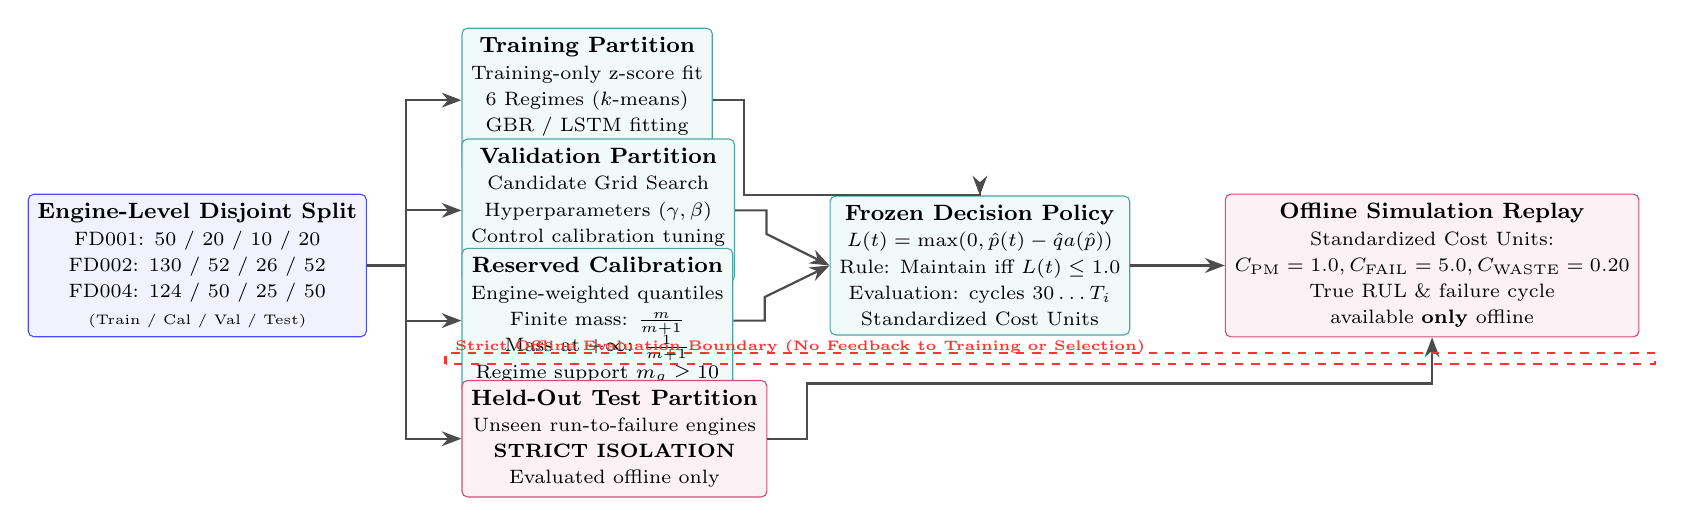
\begin{tikzpicture}[
    node distance=1.1cm and 0.8cm,
    box/.style={rectangle, draw=black!70, rounded corners=2pt, minimum width=2.5cm, minimum height=0.9cm, align=center, font=\footnotesize},
    databox/.style={rectangle, draw=blue!70, fill=blue!5, rounded corners=2pt, minimum width=2.7cm, minimum height=1.0cm, align=center, font=\footnotesize},
    procbox/.style={rectangle, draw=teal!70, fill=teal!5, rounded corners=2pt, minimum width=2.7cm, minimum height=1.0cm, align=center, font=\footnotesize},
    evalbox/.style={rectangle, draw=purple!70, fill=purple!5, rounded corners=2pt, minimum width=2.7cm, minimum height=1.0cm, align=center, font=\footnotesize},
    arrow/.style={-{Stealth[length=2.5mm]}, thick, draw=black!70},
    dashedarrow/.style={-{Stealth[length=2.5mm]}, thick, dashed, draw=red!70}
]

% 1. Dataset Partition Layer
\node[databox] (split) {
    \textbf{Engine-Level Disjoint Split}\\
    \scriptsize FD001: 50 / 20 / 10 / 20\\
    \scriptsize FD002: 130 / 52 / 26 / 52\\
    \scriptsize FD004: 124 / 50 / 25 / 50\\
    \tiny (Train / Cal / Val / Test)
};

% 2. Partition Nodes
\node[procbox, right=1.2cm of split, yshift=2.1cm] (train) {
    \textbf{Training Partition}\\
    \scriptsize Training-only z-score fit\\
    \scriptsize 6 Regimes ($k$-means)\\
    \scriptsize GBR / LSTM fitting\\
    \scriptsize Target: $\min(\text{rul}, 125)$
};

\node[procbox, right=1.2cm of split, yshift=0.7cm] (val) {
    \textbf{Validation Partition}\\
    \scriptsize Candidate Grid Search\\
    \scriptsize Hyperparameters ($\gamma, \beta$)\\
    \scriptsize Control calibration tuning\\
    \scriptsize Zero test leakage
};

\node[procbox, right=1.2cm of split, yshift=-0.7cm] (cal) {
    \textbf{Reserved Calibration}\\
    \scriptsize Engine-weighted quantiles\\
    \scriptsize Finite mass: $\frac{m}{m+1}$\\
    \scriptsize Mass at $+\infty$: $\frac{1}{m+1}$\\
    \scriptsize Regime support $m_g \ge 10$
};

\node[evalbox, right=1.2cm of split, yshift=-2.2cm] (test) {
    \textbf{Held-Out Test Partition}\\
    \scriptsize Unseen run-to-failure engines\\
    \scriptsize \textbf{STRICT ISOLATION}\\
    \scriptsize Evaluated offline only
};

% 3. Decision & Simulator Layer
\node[procbox, right=1.2cm of val, yshift=-0.7cm] (policy) {
    \textbf{Frozen Decision Policy}\\
    \scriptsize $L(t) = \max(0, \hat{p}(t) - \hat{q} a(\hat{p}))$\\
    \scriptsize Rule: Maintain iff $L(t) \le 1.0$\\
    \scriptsize Evaluation: cycles $30 \dots T_i$\\
    \scriptsize Standardized Cost Units
};

\node[evalbox, right=1.2cm of policy] (sim) {
    \textbf{Offline Simulation Replay}\\
    \scriptsize Standardized Cost Units:\\
    \scriptsize $C_{\text{PM}}=1.0, C_{\text{FAIL}}=5.0, C_{\text{WASTE}}=0.20$\\
    \scriptsize True RUL \& failure cycle\\
    \scriptsize available \textbf{only} offline
};

% Connections
\draw[arrow] (split.east) -- ++(0.5,0) |- (train.west);
\draw[arrow] (split.east) -- ++(0.5,0) |- (val.west);
\draw[arrow] (split.east) -- ++(0.5,0) |- (cal.west);
\draw[arrow] (split.east) -- ++(0.5,0) |- (test.west);

\draw[arrow] (train.east) -| ++(0.4,-1.2) -| (policy.north);
\draw[arrow] (val.east) -| ++(0.4,-0.3) -- (policy.west);
\draw[arrow] (cal.east) -| ++(0.4,0.3) -- (policy.west);
\draw[arrow] (test.east) -| ++(0.5,0.7) -| (sim.south);
\draw[arrow] (policy.east) -- (sim.west);

% Anti-leakage boundary
\draw[dashed, red!80, line width=0.9pt] ($(test.north west)+(-0.2,0.2)$) rectangle ($(sim.south east)+(0.2,-0.2)$);
\node[red!80, font=\tiny\bfseries, above right] at ($(test.north west)+(-0.2,0.2)$) {Strict Offline Evaluation Boundary (No Feedback to Training or Selection)};

\end{tikzpicture}
\caption{End-to-End System Architecture: Data Ingestion, Base Model Training, Reserved Conformal Calibration, Frozen Decision Policy, and Isolated Held-Out Offline Evaluation.}
\label{fig:architecture}
\end{figure}

\begin{figure}[htbp]
\centering
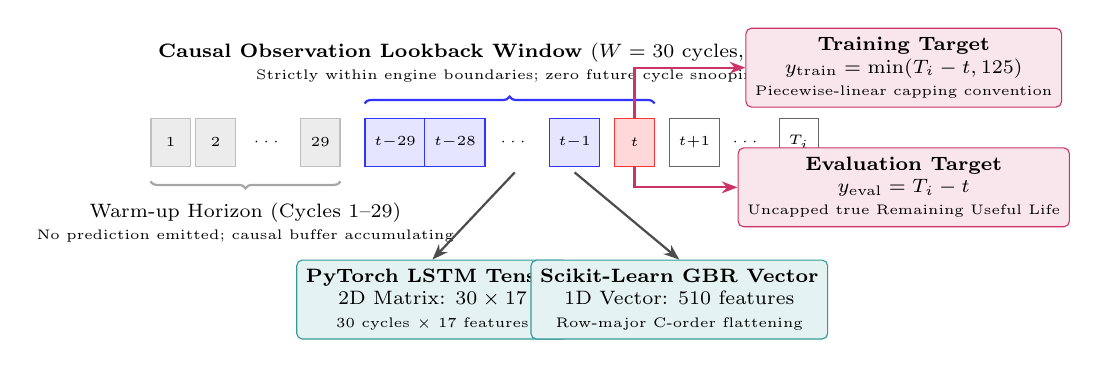
\begin{tikzpicture}[
    scale=0.95,
    cyclebox/.style={rectangle, draw=black!60, minimum width=0.5cm, minimum height=0.6cm, align=center, font=\tiny},
    warmupbox/.style={rectangle, draw=gray!50, fill=gray!15, minimum width=0.5cm, minimum height=0.6cm, align=center, font=\tiny},
    windowbox/.style={rectangle, draw=blue!80, fill=blue!10, minimum width=0.5cm, minimum height=0.6cm, align=center, font=\tiny},
    endpointbox/.style={rectangle, draw=red!80, fill=red!15, minimum width=0.5cm, minimum height=0.6cm, align=center, font=\tiny\bfseries},
    targetbox/.style={rectangle, draw=purple!80, fill=purple!10, rounded corners=2pt, minimum width=2.5cm, minimum height=0.7cm, align=center, font=\scriptsize},
    repbox/.style={rectangle, draw=teal!80, fill=teal!10, rounded corners=2pt, minimum width=2.6cm, minimum height=0.8cm, align=center, font=\scriptsize},
    arrow/.style={-{Stealth[length=2mm]}, thick, draw=black!70}
]

% Timeline coordinates
% Warm-up cycles 1, 2, ..., 28, 29
\node[warmupbox] (c1) at (0,0) {1};
\node[warmupbox] (c2) at (0.6,0) {2};
\node[font=\tiny] at (1.3,0) {$\cdots$};
\node[warmupbox] (c29) at (2.0,0) {29};

% Window cycles t-29 ... t
\node[windowbox] (ct29) at (3.0,0) {\tiny $t{-}29$};
\node[windowbox] (ct28) at (3.8,0) {\tiny $t{-}28$};
\node[font=\tiny] at (4.6,0) {$\cdots$};
\node[windowbox] (ct1) at (5.4,0) {\tiny $t{-}1$};
\node[endpointbox] (ct) at (6.2,0) {$t$};

% Next cycles
\node[cyclebox] (ctplus) at (7.0,0) {\tiny $t{+}1$};
\node[font=\tiny] at (7.7,0) {$\cdots$};
\node[cyclebox] (cT) at (8.4,0) {$T_i$};

% Labels and Braces
\draw[thick, decoration={brace, mirror, raise=4pt}, decorate, draw=gray!70] 
    ($(c1.south west)+(0,-0.05)$) -- ($(c29.south east)+(0,-0.05)$) 
    node[pos=0.5, below=8pt, font=\scriptsize, align=center] {Warm-up Horizon (Cycles 1--29)\\ \tiny No prediction emitted; causal buffer accumulating};

\draw[thick, decoration={brace, raise=4pt}, decorate, draw=blue!80] 
    ($(ct29.north west)+(0,0.05)$) -- ($(ct.north east)+(0,0.05)$) 
    node[pos=0.5, above=8pt, font=\scriptsize, align=center] {\textbf{Causal Observation Lookback Window} ($W = 30$ cycles, Stride = 1)\\ \tiny Strictly within engine boundaries; zero future cycle snooping};

% Feature Representation Nodes below
\node[repbox] (lstm_rep) at (3.5, -2.1) {
    \textbf{PyTorch LSTM Tensor}\\
    \scriptsize 2D Matrix: $30 \times 17$\\
    \tiny 30 cycles $\times$ 17 features
};

\node[repbox] (gbr_rep) at (6.8, -2.1) {
    \textbf{Scikit-Learn GBR Vector}\\
    \scriptsize 1D Vector: $510$ features\\
    \tiny Row-major C-order flattening
};

\draw[arrow] (4.6, -0.4) -- (lstm_rep.north);
\draw[arrow] (5.4, -0.4) -- (gbr_rep.north);

% Target nodes attached to endpoint t
\node[targetbox] (train_target) at (9.8, 1.0) {
    \textbf{Training Target}\\
    \scriptsize $y_{\text{train}} = \min(T_i - t, 125)$\\
    \tiny Piecewise-linear capping convention
};

\node[targetbox] (eval_target) at (9.8, -0.6) {
    \textbf{Evaluation Target}\\
    \scriptsize $y_{\text{eval}} = T_i - t$\\
    \tiny Uncapped true Remaining Useful Life
};

\draw[arrow, draw=purple!80] (ct.north) |- (train_target.west);
\draw[arrow, draw=purple!80] (ct.south) |- (eval_target.west);

\end{tikzpicture}
\caption{Causal Sliding Lookback Window Construction ($W = 30$), Dual Feature Representation Mappings (LSTM $30 \times 17$ vs. GBR $510$), and Training vs. Evaluation Target Formulations.}
\label{fig:causal_window}
\end{figure}

\begin{figure}[htbp]
\centering
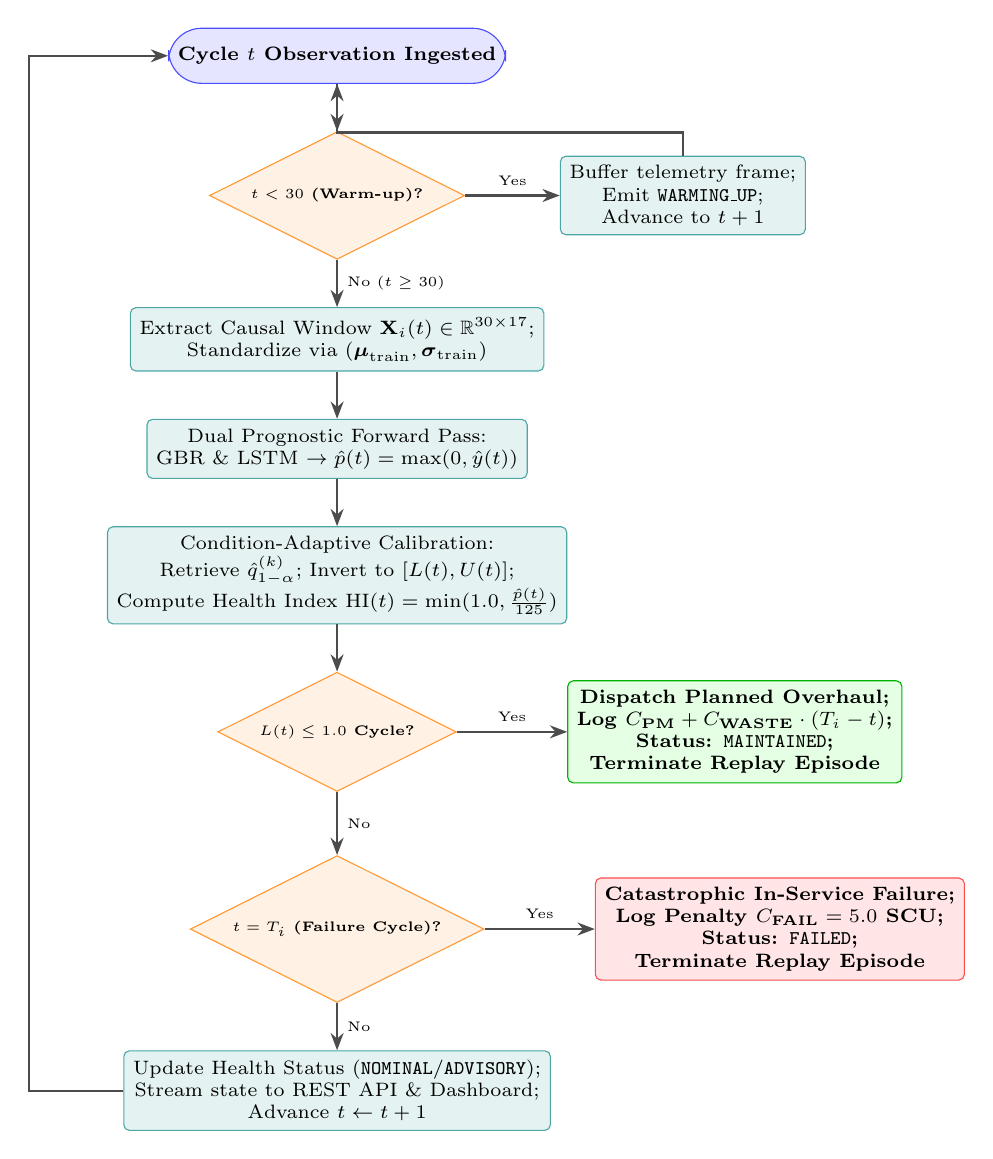
\begin{tikzpicture}[
    node distance=0.8cm and 0.6cm,
    startstop/.style={rectangle, rounded corners=12pt, draw=blue!70, fill=blue!10, minimum width=2.4cm, minimum height=0.7cm, align=center, font=\scriptsize\bfseries},
    process/.style={rectangle, draw=teal!70, fill=teal!10, rounded corners=2pt, minimum width=3.0cm, minimum height=0.75cm, align=center, font=\scriptsize},
    decision/.style={diamond, draw=orange!80, fill=orange!10, aspect=2, minimum width=2.2cm, minimum height=0.8cm, align=center, font=\tiny\bfseries},
    actionbox/.style={rectangle, draw=green!70!black, fill=green!10, rounded corners=2pt, minimum width=2.8cm, minimum height=0.75cm, align=center, font=\scriptsize\bfseries},
    failbox/.style={rectangle, draw=red!70, fill=red!10, rounded corners=2pt, minimum width=2.8cm, minimum height=0.75cm, align=center, font=\scriptsize\bfseries},
    arrow/.style={-{Stealth[length=2.2mm]}, thick, draw=black!70}
]

\node[startstop] (start) {Cycle $t$ Observation Ingested};
\node[decision, below=0.6cm of start] (warmup) {$t < 30$ (Warm-up)?};
\node[process, right=1.2cm of warmup] (defer) {Buffer telemetry frame;\\Emit \texttt{WARMING\_UP};\\Advance to $t+1$};
\node[process, below=0.6cm of warmup] (window) {Extract Causal Window $\mathbf{X}_i(t) \in \mathbb{R}^{30 \times 17}$;\\Standardize via $(\boldsymbol{\mu}_{\text{train}}, \boldsymbol{\sigma}_{\text{train}})$};
\node[process, below=0.6cm of window] (infer) {Dual Prognostic Forward Pass:\\GBR \& LSTM $\to \hat{p}(t) = \max(0, \hat{y}(t))$};
\node[process, below=0.6cm of infer] (conformal) {Condition-Adaptive Calibration:\\Retrieve $\hat{q}_{1-\alpha}^{(k)}$; Invert to $[L(t), U(t)]$;\\Compute Health Index $\text{HI}(t) = \min(1.0, \frac{\hat{p}(t)}{125})$};
\node[decision, below=0.6cm of conformal] (check_pm) {$L(t) \le 1.0$ Cycle?};

\node[actionbox, right=1.4cm of check_pm] (pm_act) {Dispatch Planned Overhaul;\\Log $C_{\text{PM}} + C_{\text{WASTE}} \cdot (T_i - t)$;\\Status: \texttt{MAINTAINED};\\Terminate Replay Episode};

\node[decision, below=0.8cm of check_pm] (check_fail) {$t = T_i$ (Failure Cycle)?};

\node[failbox, right=1.4cm of check_fail] (fail_act) {Catastrophic In-Service Failure;\\Log Penalty $C_{\text{FAIL}} = 5.0$ SCU;\\Status: \texttt{FAILED};\\Terminate Replay Episode};

\node[process, below=0.6cm of check_fail] (advance) {Update Health Status (\texttt{NOMINAL}/\texttt{ADVISORY});\\Stream state to REST API \& Dashboard;\\Advance $t \leftarrow t + 1$};

% Arrows
\draw[arrow] (start) -- (warmup);
\draw[arrow] (warmup) -- node[above, font=\tiny] {Yes} (defer);
\draw[arrow] (defer) |- ++(0,0.8) -| (start);
\draw[arrow] (warmup) -- node[right, font=\tiny] {No ($t \ge 30$)} (window);
\draw[arrow] (window) -- (infer);
\draw[arrow] (infer) -- (conformal);
\draw[arrow] (conformal) -- (check_pm);
\draw[arrow] (check_pm) -- node[above, font=\tiny] {Yes} (pm_act);
\draw[arrow] (check_pm) -- node[right, font=\tiny] {No} (check_fail);
\draw[arrow] (check_fail) -- node[above, font=\tiny] {Yes} (fail_act);
\draw[arrow] (check_fail) -- node[right, font=\tiny] {No} (advance);
\draw[arrow] (advance.west) -- ++(-1.2,0) |- (start.west);

\end{tikzpicture}
\caption{Cycle-by-Cycle Digital Twin Replay Engine and Sequential Maintenance Decision Workflow.}
\label{fig:twin_workflow}
\end{figure}

\begin{thebibliography}{14}
\bibitem{saxena2008damage} A. Saxena, K. Goebel, D. Simon, and N. Eklund, "Damage propagation modeling for aircraft engine run-to-failure simulation," in \textit{Proc. 2008 Int. Conf. Prognostics and Health Management (PHM)}, IEEE, 2008, pp. 1--9.
\bibitem{huang2021survey} Z. Huang, Y. Shen, J. Li, M. Fey, and C. Brecher, "A survey on AI-driven digital twins in Industry 4.0: Smart manufacturing and advanced robotics," \textit{Sensors}, vol. 21, no. 19, p. 6340, 2021.
\bibitem{diao2026turbofan} R. Diao, M. Zhou, G. Meng, and S. Wang, "Turbofan engine remaining useful life prediction with reliable prediction intervals via LSTM-based quantile regression and conformal calibration," \textit{Sensors}, vol. 26, no. 7, p. 2249, 2026.
\bibitem{javanmardi2023conformal} A. Javanmardi and E. H{\"u}llermeier, "Conformal prediction intervals for remaining useful lifetime estimation," \textit{Int. J. Progn. Health Manag.}, vol. 14, no. 2, pp. 1--14, 2023.
\bibitem{zhu2025predictive} Z. Zhu, L. Wang, M. Chen, and X. Zhao, "Predictive maintenance strategies for aero-engines considering remaining useful life prediction interval," \textit{Qual. Reliab. Eng. Int.}, 2025, doi: 10.1002/qre.70043.
\bibitem{chen2022data} C. Chen, J. Shi, N. Lu, Z. H. Zhu, and B. Jiang, "Data-driven predictive maintenance strategy considering the uncertainty in remaining useful life prediction," \textit{Neurocomputing}, vol. 494, pp. 79--88, 2022.
\bibitem{cortesgomez2025utility} S. Cortes-Gomez, C. M. Pati{\~n}o, Y. Byun, S. Wu, E. Horvitz, and B. Wilder, "Utility-directed conformal prediction: A decision-aware framework for actionable uncertainty quantification," in \textit{Int. Conf. Learn. Represent. (ICLR)}, 2025.
\bibitem{walia2026uncertainty} G. K. Walia and M. Kumar, "Uncertainty-aware remaining useful life prediction and PPO based optimal maintenance scheduling in industrial IoT," \textit{Reliab. Eng. Syst. Saf.}, p. 112356, 2026.
\bibitem{lee2023hierarchical} Y. Lee, R. F. Barber, and R. Willett, "Distribution-free inference with hierarchical data," \textit{arXiv preprint arXiv:2306.06342}, 2023.
\bibitem{robinson2026riskaware} C. D. Robinson, "Remaining useful life estimation for aircraft engines with risk-aware prediction intervals via conformalized quantile regression," \textit{Int. J. Progn. Health Manag.}, vol. 17, no. 1, p. 4724, 2026.
\bibitem{gneiting2007strictly} T. Gneiting and A. E. Raftery, "Strictly proper scoring rules, prediction, and estimation," \textit{J. Am. Stat. Assoc.}, vol. 102, no. 477, pp. 359--378, 2007.
\bibitem{lakens2017equivalence} D. Lakens, "Equivalence tests: A practical primer for t tests, correlations, and meta-analyses," \textit{Soc. Psychol. Personal. Sci.}, vol. 8, no. 4, pp. 355--362, 2017.
\bibitem{wu2026research} J. Wu, Y. Zhou, X. Wang, C. Chen, Y. Ma, and C. Zhang, "Research on remaining useful life prediction of equipment based on digital twins," \textit{Sensors}, vol. 26, no. 4, p. 1240, 2026.
\bibitem{iso23247} ISO 23247-1:2021, "Automation systems and integration — Digital twin framework for manufacturing — Part 1: Overview and general principles," International Organization for Standardization, Geneva, Switzerland, 2021.
\end{thebibliography}

\end{document}

